\chapter{Global Navigation Satellite Systems}
Progress in space sciences and an increasing interest in the exploration of the universe caused that nowadays many satellites
are present at the Earth's orbit and used in different fields of our
lives such as telecommunication, meteorology or environmental monitoring. Design of the Doppler TRANSIT system (Navy 
Navigation Satellite System) by the United States Navy, and making it available to the public, started the era of satellite 
positioning.
Experiences that had been gathered during the TRANSIT era were utilized in the establishment and development of 
the Navigation Satellite and Ranging Global Positioning System (NAVSTAR GPS). The latter system completely replaced its forerunner 
in the end of 1996~\citep{Teunissen:2017}. Currently, GPS serves millions of users around the globe and finds its applications in 
science and industry. It is one of the two fully operational global navigation satellite systems (Tab.~\ref{tab:GNSSconstelations}). 
Nowadays, GLONASS (Global′naya Navigatsionaya Sputnikova Sistema) is the second positioning system in operation, with a global coverage 
and of similar precision. The fully civil GALILEO system is a project of European Union (EU) and European Space Agency (ESA). Currently, it 
is at the phase of introduction of satellites at the Earth's orbit. Future launches will bring the GALILEO constellation to its full strength of 
thirty (twenty four and six spare) satellites by 2020 when fully operational services with higher accuracy and availability will begin. 
In addition, in 2015 the Chinese navigation satellite system called BeiDou began its transition towards a global coverage.
When coping with satellite navigation systems, the term one often encounters is GNSS, which stands for the Global Navigation Satellite System. 
This is a generic name used to describe any global system of satellites that transmit signals for navigation purposes. \par{}

\begin{minipage}{\textwidth}
{Tab.1~Global and regional navigation satellite systems.} \\
\footnotesize
\begin{tabular}{ c c c c c l  }
\textbf{System} & \textbf{Owner}   &  \makecell{\textbf{Intended}  \\ \textbf{coverage} \\ \textbf{ area} }   &   \makecell{\textbf{Orbital} \\ \textbf{altitude [km]}}   &  \makecell{\textbf{No. and type} \\ \textbf{of operational} \\ \textbf{satellites\footnote{Valid at \today}} }  &    \makecell{\textbf{Frequency} \\ \textbf{ bands [MHz]}}\\
 \hline\hline
 \textbf{GPS} & \makecell{United \\ States}  & Global & 20 180   & 31\footnote{The full constellation consists of 24 satellites} MEO\footnote{Medium Earth Orbit} & \makecell{1575.42 (L1) \\ 1227.60 (L2) \\ 1176.45 (L5)}  \\
\hline
  \textbf{GLONASS}&  \makecell{Russian \\ Federation}  & Global  &  19 139 & 23 MEO & \makecell{1598.0625--1605.375 (G1) \\ 1142.9375--1248.625 (G2) \\ 1201.743--1207.242 (G3)} \\
  \hline
 \textbf{GALILEO} & EU and ESA & Global  & 23 222 & 14 MEO  & \makecell{1575.42 (E1) \\  1176.45 (E5a) \\  1207.14 (E5b) \\  1278.75 (E6)} \\
  \hline
  \textbf{BeiDou} & China & Global  & 21 150 & \makecell{4 MEO \\  7 GEO\footnote{Geostationary Orbit} \\ 6 GSO\footnote{Geosynchronous Orbit} } & \makecell{1561.098/1589.42/2575.42 (B1) \\ 1589.742 (B1-2) \\ 1207.140 (B2) \\ 1268.52 (B3) }\\
 \hline
\textbf{IRNSS}  & India  & Regional  & 36 000    &  \makecell{4 GSO \\ 3 GEO}& \makecell{1176.45 (L5) \\ 2492.03 (S1)}  \\
\hline
\textbf{QZSS}   & Japan & Regional  &\makecell{32 000 \\ -- \\ 40 000}  &  1 GSO   & \makecell{1575.42 (L1) \\ 1227.60 (L2) \\ 1176.45 (L5) \\ 1278.75 (E6)} \\
\\ 

\end{tabular}
  \label{tab:GNSSconstelations}
%\end{table}
\end{minipage}
Each of the navigation satellite systems consists of space, control and user segments. The space segment comprises satellites 
located at few orbits and transmitting signals between 1.2 and 1.6 GHz (a part of the so-called L-band). 
The control segment is a group of ground-based stations, which monitor the space segment in order to 
know very precisely where the satellites were, are and will be in the future. The last segment includes civil as well 
as military users equipped with GNSS receivers. Depending on the equipment type, users can determine their position with 
different precision in real time or during the post-­processing of observations recorded over periods of hours or days~\citep{Teunissen:2017}. \par{}

Satellite positioning finds its applications not only in navigation and timing services, but also in the interdisciplinary 
research on Earth. GPS has introduced significant changes in the process of monitoring of the movement of tectonic plates or horizontal and 
vertical deformation of the Earth's crust caused by e.g. melting glaciers or earthquakes~\citep{Wake2016}. In the last few microseconds 
of their journey, the incoming GNSS (radio) signals 
encounter propagation effects while passing through the atmosphere. This knowledge can be quantified and utilized in meteorological observations 
and atmospheric studies. Moreover, GNSS does not only reveal geophysical phenomena in space and time, but also contributes to the establishment and 
maintenance of global reference frames, which the observed phenomena and their spatio-temporal variability can be properly referenced to~\citep{AltamimiITRF2014}. 

%\begin{figure*}[h!] 
%\centering
%\includegraphics[width=0.8\textwidth]{\plotFolder/GNSSsegments.png}
%\caption{GNSS segments \citep{}} 
%\label{fig:GNSSsegments}
%\end{figure*}

\section{GNSS signals}

GNSS signals are electromagnetic waves propagating at the speed of light. An oscillator located on the board of a GNSS satellite generates the fundamental 
frequency $f_0$ which is then used to generate radio signals that are sent 
towards the Earth. GNSS signals are created through the multiplication of $f_0$ by different predefined integer values\footnote{In the case of GPS L1 band, this is $154 \times 10.23\,\textrm{MHz}$ 
which gives 1575.42~MHz. For GPS L2 the integer value amounts to 120 which gives 1227.60~MHz.}. Each GNSS system provides signals on at least two different frequencies in 
order to deal with the signal delay caused by the ionosphere. In order to convey digital data, the generated signals are also modified by changing (modulating) their 
phase. In the case of the biphase modulation (BPSK) there will be a 180\deg shift in the phase of the signal whenever a change in the value of the bit (symbol) will appear (Fig.~\ref{fig:SignalModulation}).
In each satellite 
navigation system, the aforementioned digital data consist of ranging codes and downlink system data codes (broadcast navigation message). Ranging codes are used to estimate 
the position of a receiver on the ground. Information such as satellite's oscillator (clock) offset from the GNSS system time, satellite's three-dimensional position, status 
messages or correction data are transmitted in the navigation message.\par{}

\begin{wrapfigure}{l}{0.4\textwidth} 
  \begin{center}
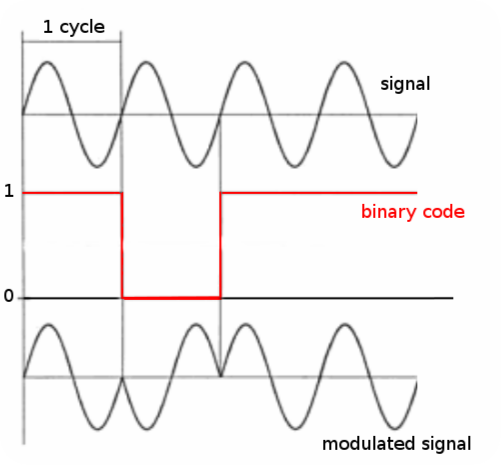
\includegraphics[width=0.4\textwidth]{\plotFolder/ModulatedSignal.png}
\caption{BPSK signal modulation.} 
    \label{fig:SignalModulation}
  \end{center}
\end{wrapfigure} 
In each navigation system satellites transmit signals with the same strength. Different power levels are assigned however to different frequency bands. As an example, 
GPS transmits on L5 with power levels reaching 263~W, whereas on L2 it is only 4~W. Users on the ground receive
signals with varying strength and that are sometimes discontinuous. A loss in the singal strength is proportional to the distance to the satellite, which means that the 
further the ground receiver is located from a satellite, the signal is weaker\footnote{This effect is known as the free-space loss ($L_{FS}$). It depends on the distance (R) from the receiver 
to a satellite and the used frequency (f): $  L_{FS} =  \left( \frac{4 \cdot \pi \cdot R \cdot f }{c} \right)^2 $, where $c$ is the speed of light. }. Signals transmitted 
on L-band do not suffer from high attenuation under harsh weather conditions, compared to e.g. signals at frequencies above 10 GHz.
A satellite signal is often diminished by radio interference or obstacles such as high buildings or trees located close to a GNSS receiver.  \par{}
Multiple ­access techniques allow to distinguish between signals transmitted by different satellites. With Code-Division Multiple Access (CDMA) it is possible to use the same frequency
spectrum by all satellites of the navigation system. In GLONASS however, Frequency-Division Multiple Access (FDMA) in both G1 and G2 bands is utilized instead. As a consequence, slightly different 
frequencies are used by each satellite\footnote{In practice, two satellites, located on antipodal sides of a single orbital plane, transmit signals using the same frequency.}. However, new generation 
of GLONASS satellites will transmit CDMA signals in addition to the system's traditional FDMA. In general, development and modernization programs of all contemporary navigation satellite 
systems aim for better accuracy, multipath resistance and especially, greater interoperability with other navigation systems.

\section{GNSS positioning principle}

The basic measurement carried out by any GNSS receiver, for navigation purposes, is the signal propagation time from a satellite
to the receiver. It is determined by comparing (correlating) the received binary code (pseudorandom noise) 
embedded in the signal with the internally-generated replica at the local receiver time~(Fig.~\ref{fig:PseudorangeMeasurements}). 
This measured quantity can be easily converted to a distance (pseudorange) by multiplying it by the speed of light and used to localize the 
receiver w.r.t the satellite, which signal was sent from. 
It is possible to determine the three-dimensional position of the receiver if it simultaneously observes signals 
coming from many satellites, which position is well known thanks to the ground segment. In principle, we would need to measure ranges to at least three satellites.
However, the internal oscillator (clock) of the receiver is mis-synchronized with respect to the satellite clocks.
Therefore, an offset of the receiver clock with respect to the system time is estimated for each observation epoch. This 
implies that one needs to have at least four satellites to be able to solve for the receiver's position with a usable accuracy. 
Satellite clocks are also not perfectly in sync with each other and the system time. This is however dealt with by estimating 
the offsets and drifts of satellite clocks with respect to the system time. These parameters are then used by GNSS receivers 
as corrections to the measured ranges. \par{}

\begin{figure}[ht]
  \begin{center}
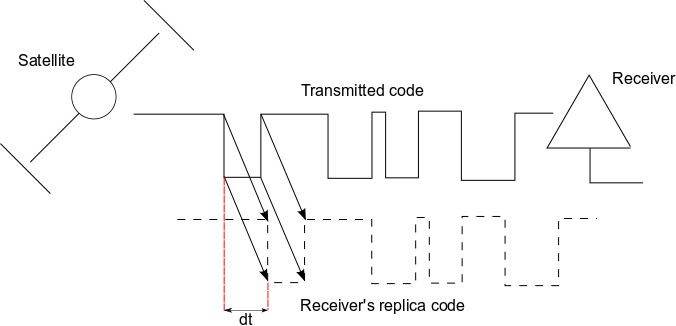
\includegraphics[width=0.75\textwidth]{\plotFolder/GNSSPseudorange.png}
\caption{GNSS pseudorange measurement principle.} 
    \label{fig:PseudorangeMeasurements}
  \end{center}
\end{figure} 

Under the assumption of receiver and satellite clocks being in sync and in the presence of no additional errors, our position uncertainty would be 
only proportional to the error in determination of the position of satellites. When one includes satellite clock
and atmospheric propagation errors as well as receiver's noise into the error budget, all
expressed in units of distance, the current positioning accuracy from range measurements amounts to few meters. This 
quantity tends to vary as it is related to e.g. the location of a GNSS receiver (cities, open fields), number of used satellites and their location on the 
local sky~\citep{Teunissen:2017}.